\documentclass[12pt]{article}

\usepackage{amsmath}
\usepackage{graphicx}
\usepackage{parskip}

\title{Balance-assist bicycle weave mode experiments: measurements and parameter adjustions}
\author{Marten Haitjema}
\date{\today}

\begin{document}
\maketitle

\section{Introduction}
Research into the balance-assist bicycle is done with a model of a bicycle. The parameters of this model are for a different bicycle than the balance-assist bicycle. It is unknown how well the model represents the balance-assist bicycle. It is important for the balance-assist bicycle to be properly modelled, because the controller is designed based on the (thus far inaccurate) model. If the model is not representative of the balance-assist bicycle, the designed controller may be invalid. 

The goal of this experiment is to identify the actual weave mode of the balance-assist bicycle for different controller gains. 

\section{Methods}
The weave mode will be identified by manually perturbing the bicycle at the seat post, and measuring the consequent roll rate. The weave mode can be found be fitting a decaying oscillation to this data. The following equation, defined by Kooijman et al. \cite{Kooijman2008}, is used to fit to the roll rate data:

\begin{equation}
    c_1 + e^{dt} (c_2\cos(\omega t) + c_3\sin(\omega t))
    \label{kooijman-func}
\end{equation}

The imaginary part of the eigenvalue is given by the frequency $\omega$. The real part is given by the damping $d$. An example of the function fitted to roll rate data can be seen in figure \ref{example-roll-rate-fit}. Eigenvalues were measured with the balance-assist system on with a gain of -6, -8 and -8 at speeds of 6, 8, 10, 12, 14, 16 and 18 km/h. For each velocity, the real and imaginary part of the eigenvalues were averaged over three perturbations.

\begin{figure}[h]
    \centering
    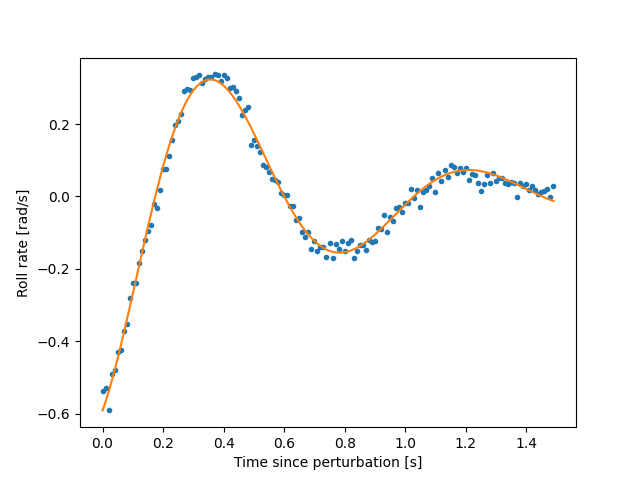
\includegraphics[width=\columnwidth]{figures/example_roll_rate_fit.png}
    \caption{Example of a fit of a decaying oscillation to roll rate data.}
    \label{example-roll-rate-fit}
\end{figure}


\section{Results}
Measured eigenvalues for a gain of -6 can be seen in figure \ref{gain-6-batavus-without-rider} and table \ref{table-eigenvalues-gain-6}. The results for a gain of -8 can be seen in figure \ref{gain-8-batavus-without-rider} and table \ref{table-eigenvalues-gain-8}. The results for a gain of -10 can be seen in figure \ref{gain-10-batavus-without-rider} and table \ref{table-eigenvalues-gain-10}.

For the gain of -6, the theoretical weave mode of the Batavus Browser bicycle with a model of the balance-assist system is close the measured eigenvalues. For the gain of -8 and -10, the measured real part of the eigenvalues is less damped than the Batavus Browser. For all gains, the imaginary part of the eigenvalues is substantially lower than the theoretical eigenvalues.


\begin{table}[]
    \centering
    \caption{Real and imaginary parts of the measured eigenvalues for a gain of -6.}
    \label{table-eigenvalues-gain-6}
    \begin{tabular}{c|c|c}
        \textbf{Velocity (m/s)} & \textbf{Real part} & \textbf{Imaginary part} \\ \hline
        1.66                    & -3.10437           & 6.90899                 \\
        2.22                    & -1.73230           & 7.47695                 \\
        2.78                    & -1.07677           & 7.81142                 \\
        3.33                    & -0.64501           & 7.79933                 \\
        3.89                    & -0.57419           & 6.93977                 \\
        4.44                    & -0.73719           & 7.33274                 \\
        5.00                    & -0.82591           & 4.65962                
    \end{tabular}
\end{table}

\begin{figure}
    \centering
    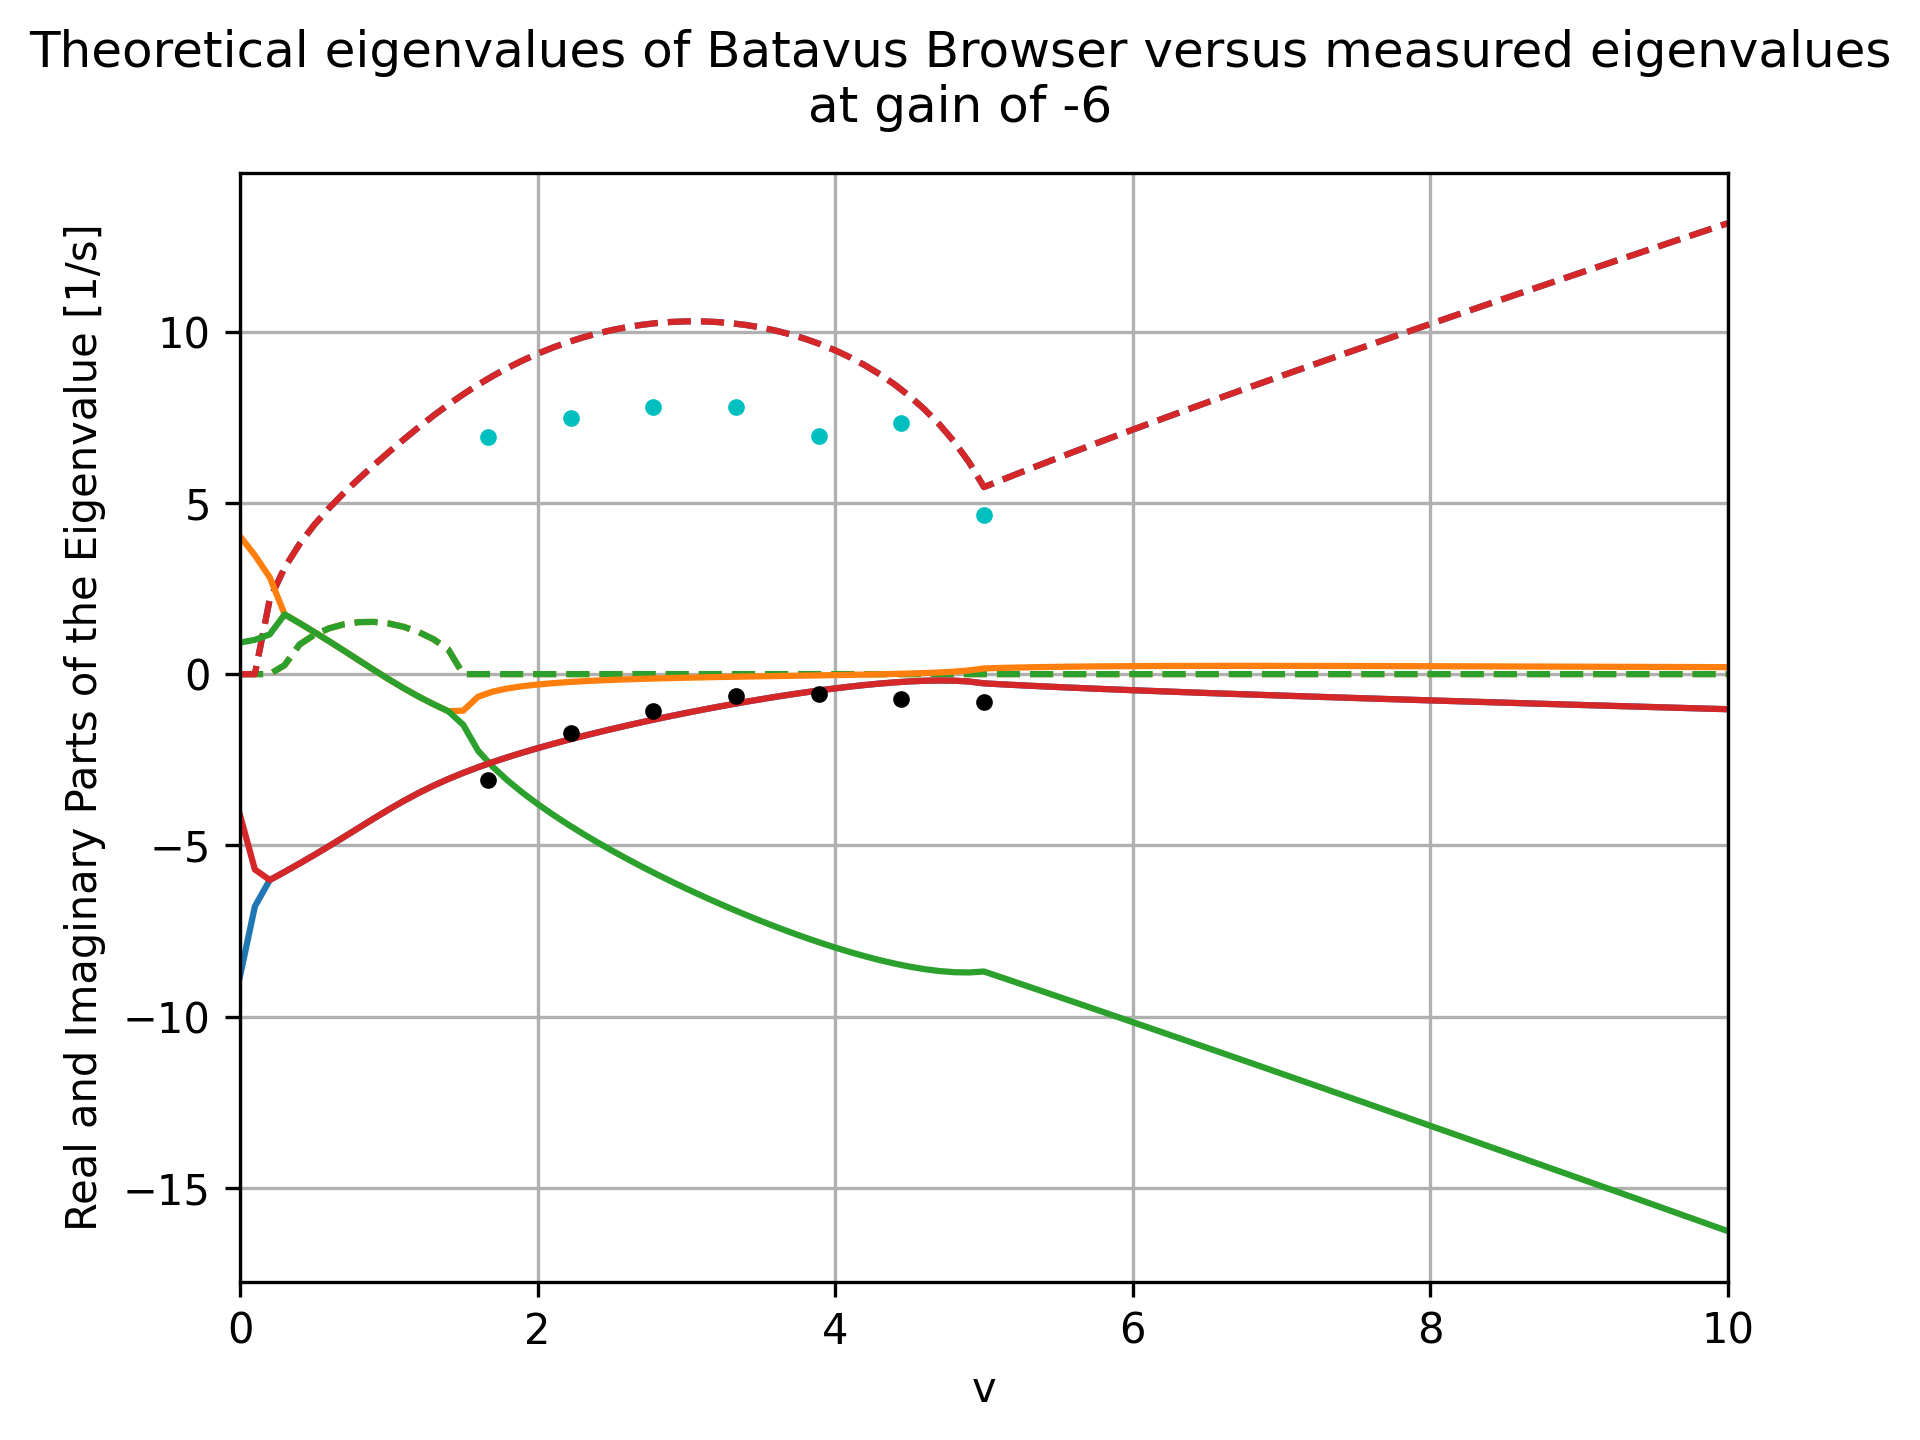
\includegraphics[width=\columnwidth]{figures/gain-6-batavus-without-rider.png}
    \caption{Theoretical eigenvalues of Batavus Browser with balance-assist controller and the measured eigenvalues at gain of -6. The real part of the measured eigenvalues is displayed in black, the imaginary part is displayed  in cyan.}
    \label{gain-6-batavus-without-rider}
\end{figure}


\begin{table}[]
    \centering
    \caption{Real and imaginary parts of the measured eigenvalues for a gain of -8.}
    \label{table-eigenvalues-gain-8}
    \begin{tabular}{c|c|c}
        \textbf{Velocity (m/s)} & \textbf{Real part} & \textbf{Imaginary part} \\ \hline
        1.66                    & -1.96625           & 8.97518                 \\
        2.22                    & -1.67178           & 9.59152                 \\
        2.78                    & -1.08789           & 9.82538                 \\
        3.33                    & -0.82441           & 9.27701                 \\
        3.89                    & -0.56166           & 8.26214                 \\
        4.44                    & -0.70618           & 5.97152                 \\
        5.00                    & -0.90672           & 5.32524                
    \end{tabular}
\end{table}

\begin{figure}
    \centering
    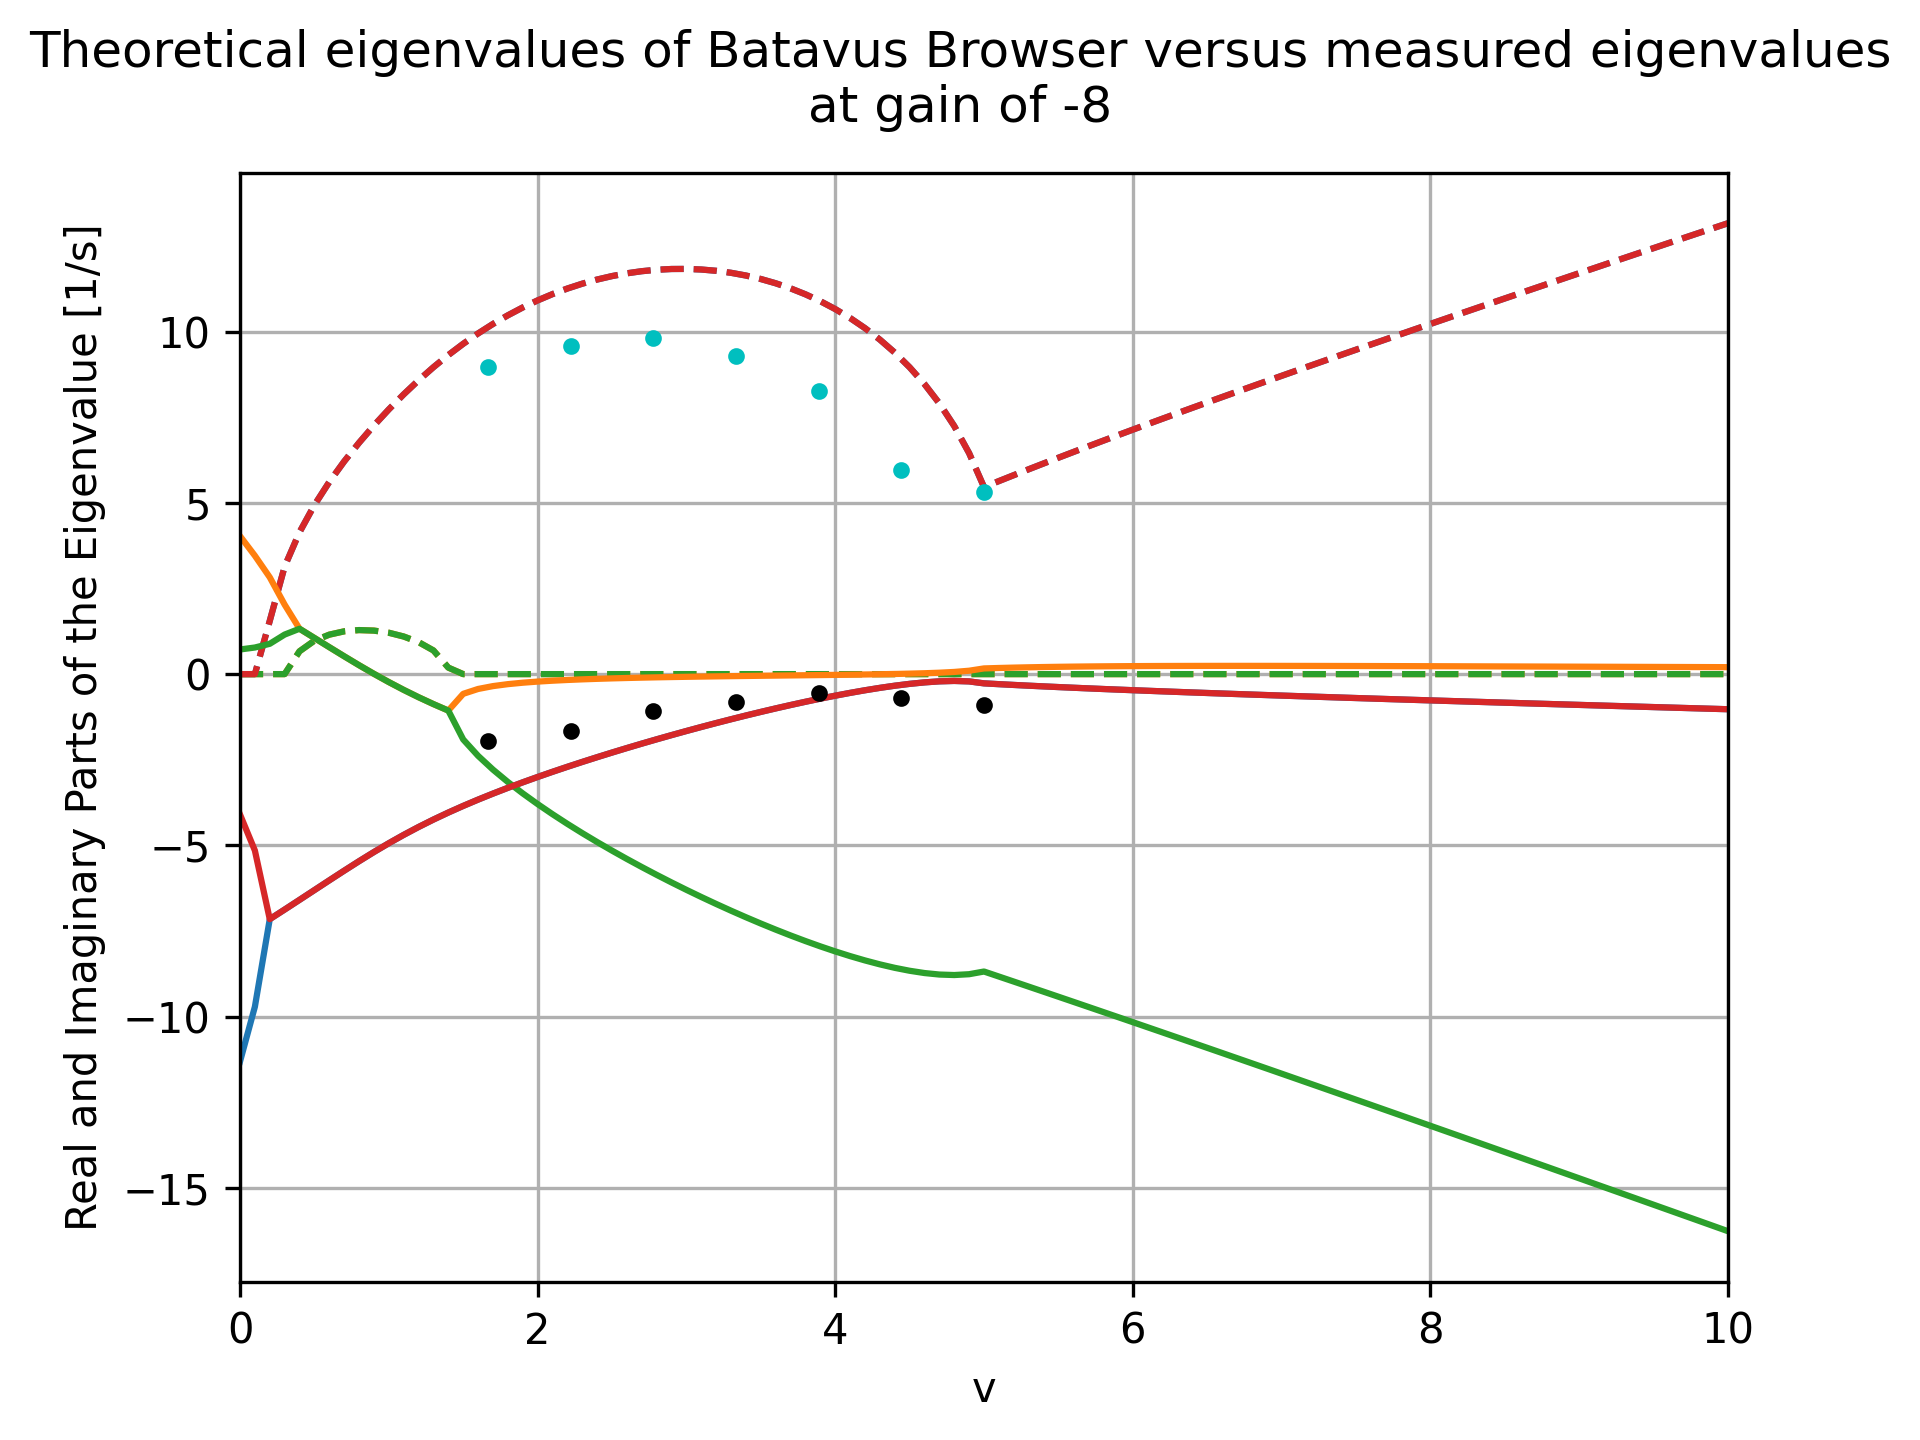
\includegraphics[width=\columnwidth]{figures/gain-8-batavus-without-rider.png}
    \caption{Theoretical eigenvalues of Batavus Browser with balance-assist controller and the measured eigenvalues at gain of -8. The real part of the measured eigenvalues is displayed in black, the imaginary part is displayed  in cyan.}
    \label{gain-8-batavus-without-rider}
\end{figure}


\begin{table}[]
    \centering
    \caption{Real and imaginary parts of the measured eigenvalues for a gain of -10.}
    \label{table-eigenvalues-gain-10}
    \begin{tabular}{c|c|c}
        \textbf{Velocity (m/s)} & \textbf{Real part} & \textbf{Imaginary part} \\ \hline
        1.66                    & -3.73303          & 11.03922                 \\
        2.22                    & -1.83437          & 10.90979                 \\
        2.78                    & -1.08183          & 10.84567                 \\
        3.33                    & -0.78383          & 10.49930                 \\
        3.89                    & -0.59061          & 9.07418                 \\
        4.44                    & -0.53405          & 6.87337                 \\
        5.00                    & -0.02263          & 4.16736                
    \end{tabular}
\end{table}

\begin{figure}
    \centering
    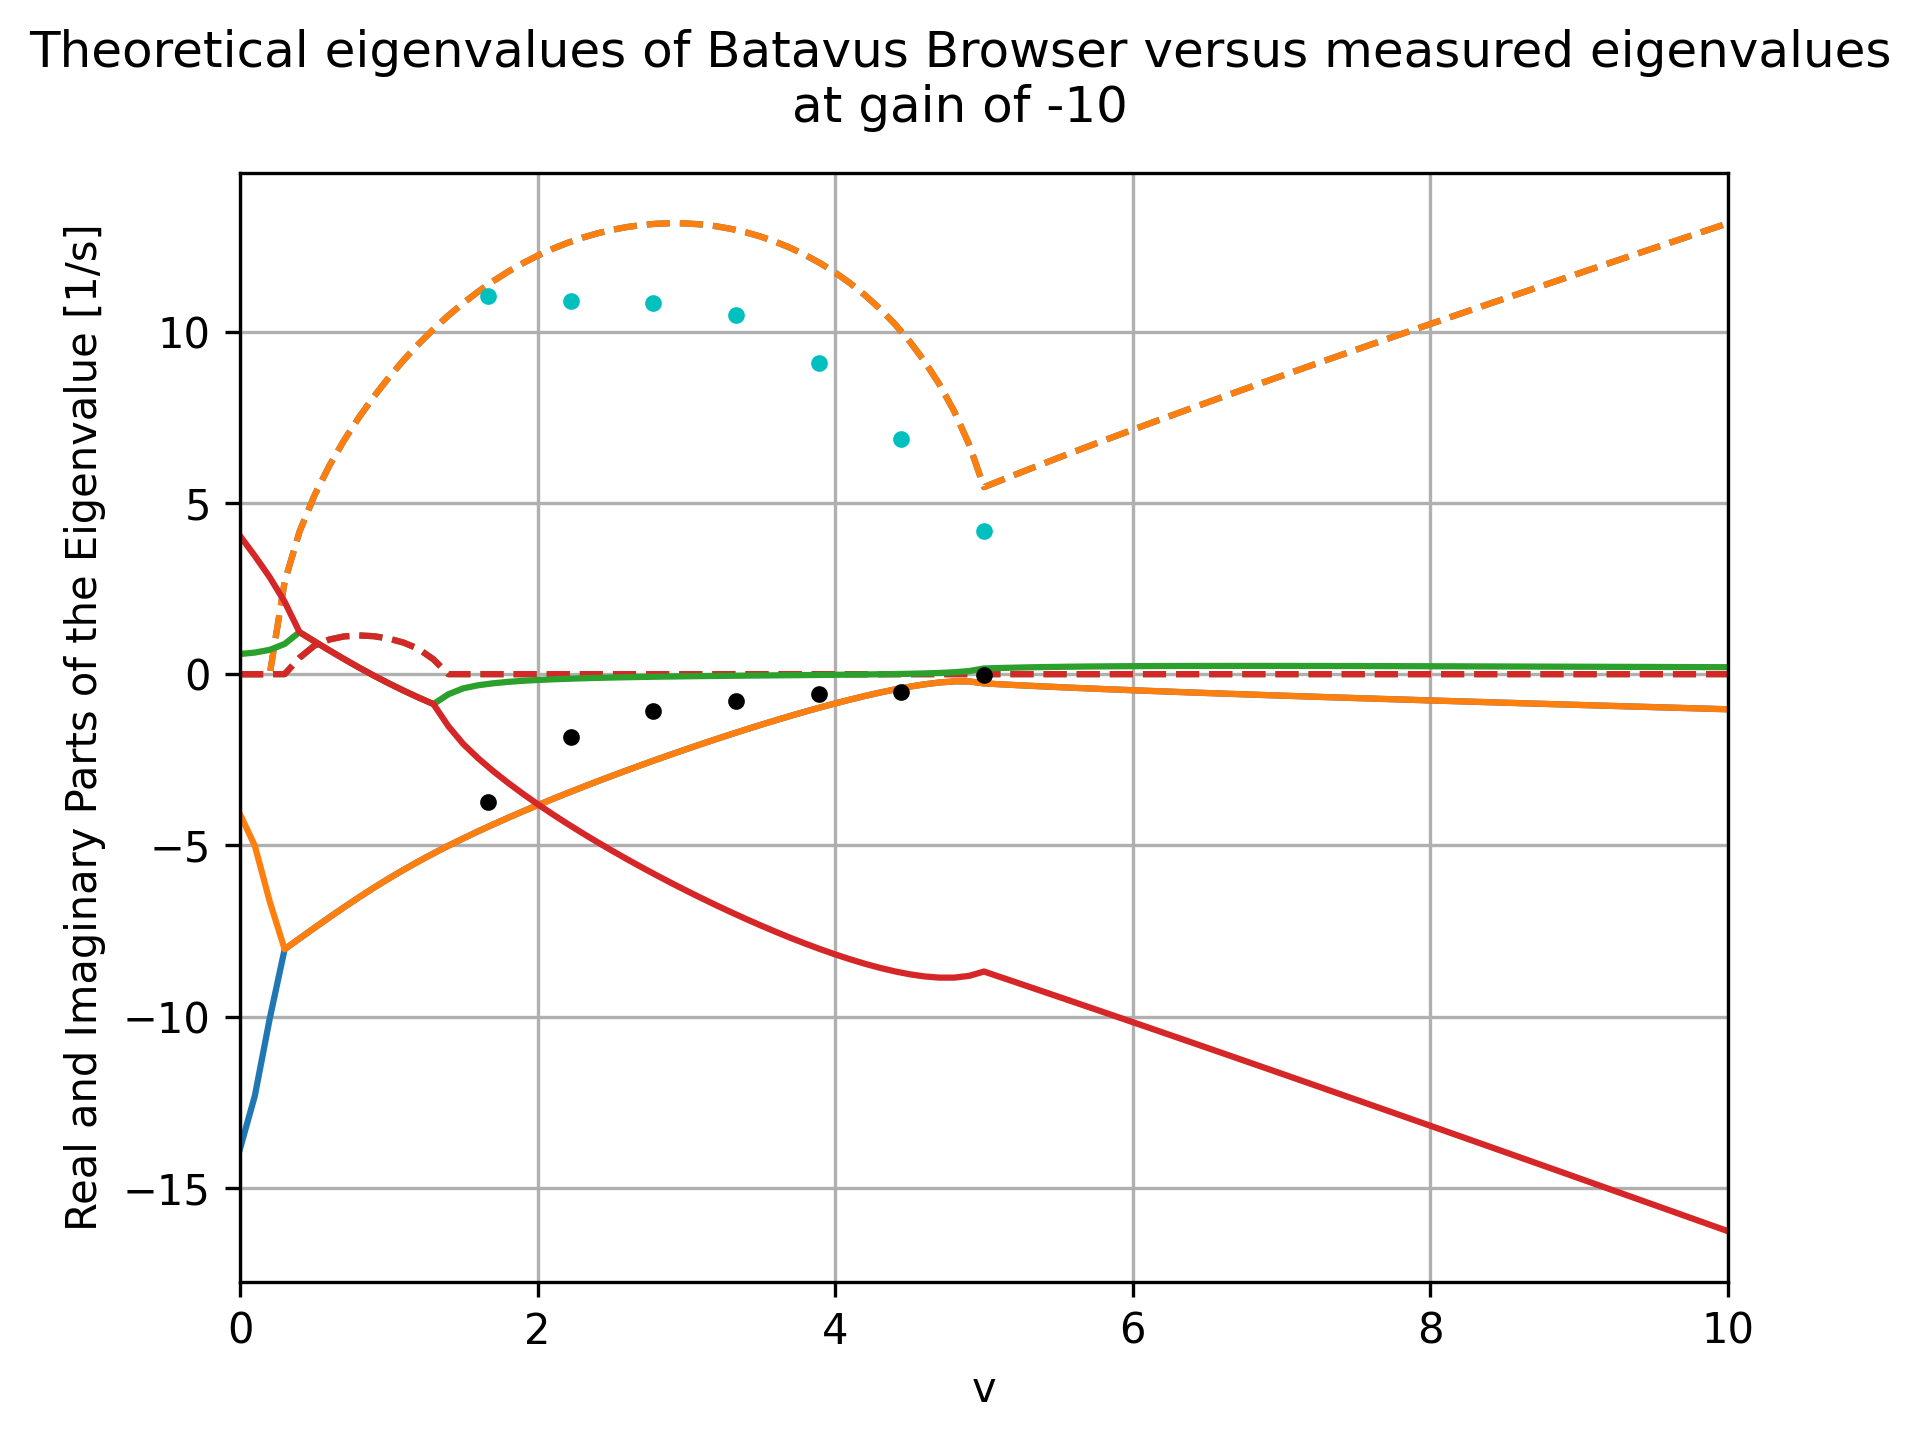
\includegraphics[width=\columnwidth]{figures/gain-10-batavus-without-rider.png}
    \caption{Theoretical eigenvalues of Batavus Browser with balance-assist controller and the measured eigenvalues at gain of -10. The real part of the measured eigenvalues is displayed in black, the imaginary part is displayed  in cyan.}
    \label{gain-10-batavus-without-rider}
\end{figure}


\section{Adjusting model parameters}
To have the model better approximate the eigenvalues of the balance-assist bicycle, the model parameters can be adjusted to better fit the measured values. The adjustments of these values should be based on the physical properties of the balance-assist bicycle. 

The balance-assist bicycle differs from the Batavus Browser bicycle in a couple of ways. First and foremost, unlike the Batavus Browser the balance-assist bicycle is electric and therefore has a heavy battery in the downtube. Moreover, the balance-assist bicycle has electronics mounted at the rear rack. These differences will influence the position of the center of mass and the mass moment of inertia. Secondly, the balance-assist bicycle has a motor at the head tube of the bicycle. This will effect the position of the center of mass and the mass moment of inertia of the front frame. In this section, an approximation of these changes will be made in order to better approach the measured eigenvalues. 

\begin{figure}
    \centering
    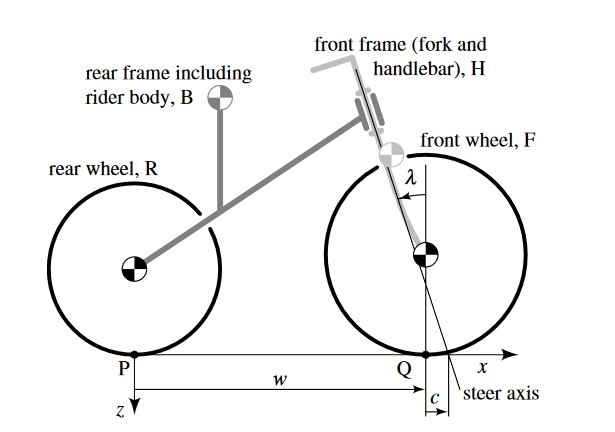
\includegraphics[width=\columnwidth]{figures/KooijmanFBD.jpg}
    \caption{Diagram of the coordinate system used to define the parameters. Note that the x-axis starts at the rear wheel ground contact point and that the positive z-axis points downwards. Adapted from Kooijman et al. \cite{Kooijman2008}.}
\end{figure}


\begin{table}[]
    \centering
    \caption{Measured parameters of the Batavus Browser and proposed parameters for the balance-assist bicycle. Only parameters that are changed are displayed.}
    \label{parameter-changes}
    \begin{tabular}{c|c|c}
        \textbf{Parameter} & \textbf{Batavus Browser} & \textbf{Balance-assist bicycle} \\ \hline
        $x_B$              & 0.275951285677           & ?                               \\
        $z_B$              & -0.537842424305          & -0.337842424305                 \\
        $I_{Bxx}$          & 0.52962890621            & ?                               \\
        $I_{Bxz}$          & -0.116285607878          & ?                               \\
        $I_{Byy}$          & 1.3163960125             & ?                               \\
        $I_{Bzz}$          & 0.756786895402           & ?                               \\
        $x_H$              & 0.866949640247           & ?                               \\
        $z_H$              & -0.748236400835          & -0.848236400835                 \\
        $I_{Hxx}$          & 0.25335539588            & ?                               \\
        $I_{Hxz}$          & -0.0720217263293         & ?                               \\
        $I_{Hyy}$          & 0.245827908036           & ?                               \\   
        $I_{Hzz}$          & 0.0955686343473          & ?
    \end{tabular}
\end{table}


\bibliographystyle{plain}
\bibliography{weave-experiments}

\end{document}